\documentclass[11pt,a4paper]{article}
\usepackage[utf8]{inputenc}
\usepackage[T1]{fontenc}
\usepackage{amsmath,amssymb,amsfonts}
\usepackage{amsthm}
\usepackage[margin=2.5cm]{geometry}
\usepackage{enumitem}
\usepackage{tikz}
\usepackage{xcolor}
\usepackage{hyperref}
\hypersetup{colorlinks=true,linkcolor=blue!55!black,urlcolor=blue!55!black}
\setlist[itemize]{leftmargin=1.4em,itemsep=2pt,topsep=3pt}

% ── theorem environments (numbered, standard) ──
\newtheorem{theorem}{Theorem}[section]
\newtheorem{lemma}[theorem]{Lemma}
\newtheorem{proposition}[theorem]{Proposition}
\newtheorem{corollary}[theorem]{Corollary}
\theoremstyle{definition}
\newtheorem{definition}[theorem]{Definition}
\newtheorem{example}[theorem]{Example}
\newtheorem{remark}[theorem]{Remark}
\newtheorem{exercise}{Exercise}

% ── master macro block (safe, multi-character) ──
\newcommand{\Z}{\mathbb{Z}}
\newcommand{\Q}{\mathbb{Q}}
\newcommand{\R}{\mathbb{R}}
\newcommand{\C}{\mathbb{C}}
\newcommand{\N}{\mathbb{N}}
\newcommand{\id}{\operatorname{id}}
\newcommand{\Deck}{\operatorname{Deck}}
\newcommand{\Sym}{\operatorname{Sym}}
\newcommand{\Aut}{\operatorname{Aut}}
\newcommand{\Gal}{\operatorname{Gal}}
\newcommand{\Spec}{\operatorname{Spec}}
\newcommand{\PP}{\mathbb{P}}

\title{
	{\color{blue!40!black}\textbf{\Huge Point}}\\[0.3em]
	\Large \textit{From Number Theory to Algebraic Geometry and Logic}\\[0.7em]
	\large \textbf{Session P3 --- Algebraic Topology Crash Course}\\[0.3em]
	\normalsize \emph{Complete lecture notes with proofs, examples, and exercises}
}
\author{}
\date{}

\begin{document}
	\maketitle
	\thispagestyle{empty}
	
	\begin{abstract}
		\noindent
		This session supplies the \emph{topological prototype of Galois theory}. We build the fundamental
		group $\pi_1(X,x_0)$, the theory of covering spaces (lifting, monodromy, deck transformations,
		universal covers), and the classification of coverings by subgroups of $\pi_1$ --- the exact
		categorical pattern that Session~S35 reproduces for schemes as Grothendieck's \'etale fundamental
		group, and that Act~VII internalizes in topoi. The dictionary at the end
		(coverings $\leftrightarrow$ field extensions, deck groups $\leftrightarrow$ Galois groups,
		universal cover $\leftrightarrow$ separable closure) is the bridge the whole course walks across.
		Scope: no homology, no higher homotopy --- just enough to make \'etale $\pi_1$ intuitive.
	\end{abstract}
	
	\subsection*{Session plan (150 minutes)}
	\begin{center}\small
		\begin{tabular}{|l|l|}
			\hline
			\textbf{Time} & \textbf{Block} \\
			\hline
			0:00--0:10 & Orientation: why coverings are the prototype of Galois theory \\
			0:10--0:40 & \S1 Homotopy and $\pi_1$: definitions, basepoint change, contractible, products \\
			0:40--1:05 & \S2 Coverings: lifting, monodromy, deck transformations \\
			1:05--1:15 & \emph{Break} \\
			1:15--1:40 & \S2 cont.: universal covers; classification; $\pi_1(S^1)\cong\Z$ \\
			1:40--2:10 & \S3 The topological Galois correspondence; the dictionary; bridge to S16, S34, S35 \\
			2:10--2:30 & Exercises / wrap-up: monodromy $=$ evaluation along loops \\
			\hline
		\end{tabular}
	\end{center}
	
	\subsection*{Conventions}
	All spaces are path-connected and locally path-connected unless stated; maps are continuous.
	$[0,1]$ carries the subspace topology of $\R$. Loops are paths with $\gamma(0)=\gamma(1)=x_0$.
	We write $S^1=\{z\in\C:|z|=1\}$ and $T^2=S^1\times S^1$.
	
	\tableofcontents
	\newpage
	
	% ══════════════════════════════════════════════
	\section{Homotopy and the Fundamental Group}
	% ══════════════════════════════════════════════
	
	\begin{definition}[Path; path homotopy]
		A \textbf{path} in $X$ from $a$ to $b$ is a continuous $\gamma:[0,1]\to X$ with $\gamma(0)=a$,
		$\gamma(1)=b$. A \textbf{path homotopy} (rel endpoints) between $\gamma_0,\gamma_1$ is a continuous
		$H:[0,1]\times[0,1]\to X$ with $H(s,0)=\gamma_0(s)$, $H(s,1)=\gamma_1(s)$, and
		$H(0,t)=a$, $H(1,t)=b$ for all $t$. We write $\gamma_0\simeq\gamma_1$.
	\end{definition}
	
	\begin{definition}[Fundamental group]
		A \textbf{loop} at $x_0$ is a path with $a=b=x_0$. For loops $\gamma,\eta$ define the concatenation
		\[
		(\gamma*\eta)(s)=
		\begin{cases}
			\gamma(2s), & 0\le s\le\tfrac12,\\
			\eta(2s-1), & \tfrac12\le s\le1.
		\end{cases}
		\]
		The \textbf{fundamental group} $\pi_1(X,x_0)$ is the set of path-homotopy classes $[\gamma]$ of loops
		at $x_0$, with operation $[\gamma]\cdot[\eta]=[\gamma*\eta]$.
	\end{definition}
	
	\begin{proposition}[$\pi_1$ is a group]\label{prop:pi1-group}
		The operation is well defined on homotopy classes and makes $\pi_1(X,x_0)$ a group: the identity is
		the class of the constant loop $c_{x_0}$, and the inverse of $[\gamma]$ is $[\bar\gamma]$ with
		$\bar\gamma(s)=\gamma(1-s)$.
	\end{proposition}
	\begin{proof}
		If $\gamma_0\simeq\gamma_1$ and $\eta_0\simeq\eta_1$ via $H,K$, then gluing $H$ and $K$ at $s=\tfrac12$
		gives a path homotopy $\gamma_0*\eta_0\simeq\gamma_1*\eta_1$: well-definedness. For the identity,
		given $\gamma$, the homotopy
		$H(s,t)=\gamma\big(\min\{1,\,2s/(1+t)\}\big)$? more transparently: reparametrize by a family of
		monotone maps $\varphi_t:[0,1]\to[0,1]$ with $\varphi_0(s)=\min\{2s,1\}$-type speed-ups; any two
		monotone reparametrizations fixing $0,1$ are homotopic through monotone maps, and precomposing
		$\gamma$ with such a homotopy is a path homotopy. Applying this to the speed-ups that realize
		$\gamma*c$ and $c*\gamma$ and to $(\gamma*\eta)*\kappa$ vs $\gamma*(\eta*\kappa)$ gives identity and
		associativity up to path homotopy. For inverses, $H(s,t)=\gamma\big(t\cdot\min\{2s,2-2s,1\}+(1-t)\cdot
		\text{(position)}\big)$ contracts the backtrack $\gamma*\bar\gamma$ to $c_{x_0}$: explicitly
		$H(s,t)=\gamma\big((1-t)\cdot\rho(s)\big)$ where $\rho$ traverses out-and-back; continuity is clear.
	\end{proof}
	
	\begin{proposition}[Basepoint change]\label{prop:basepoint}
		If $\alpha$ is a path from $x_0$ to $x_1$, then
		$\beta_\alpha:\pi_1(X,x_0)\to\pi_1(X,x_1)$, $[\gamma]\mapsto[\alpha^{-1}*\gamma*\alpha]$, is a well-defined
		group isomorphism, with inverse $\beta_{\alpha^{-1}}$. Hence for path-connected $X$, $\pi_1$ is
		independent of basepoint up to isomorphism.
	\end{proposition}
	\begin{proof}
		Concatenation respects path homotopy (Proposition~\ref{prop:pi1-group}), so $\beta_\alpha$ is
		well-defined; it is a homomorphism since the middle $\alpha*\alpha^{-1}$ cancels up to homotopy
		between products; $\beta_{\alpha^{-1}}\circ\beta_\alpha=[\alpha*(\alpha^{-1}*\gamma*\alpha)*\alpha^{-1}]
		=[\gamma]$ after cancelling, so they are mutually inverse.
	\end{proof}
	
	\begin{definition}[Homotopy equivalence; contractible]
		$f:X\to Y$ is a \textbf{homotopy equivalence} if $\exists g:Y\to X$ with $g\circ f\simeq\id_X$ and
		$f\circ g\simeq\id_Y$. $X$ is \textbf{contractible} if $\id_X\simeq$ a constant map.
	\end{definition}
	
	\begin{proposition}\label{prop:contractible}
		\begin{enumerate}[label=(\alph*)]
			\item Homotopic maps $f_0,f_1:X\to Y$ induce equal homomorphisms on fundamental groups (after
			adjusting basepoints along the track of the basepoint).
			\item A homotopy equivalence induces an isomorphism on $\pi_1$.
			\item Contractible spaces have trivial $\pi_1$ at every basepoint.
		\end{enumerate}
	\end{proposition}
	\begin{proof}[Proof ideas]
		(a) The homotopy $H$ between $f_0,f_1$ sends a loop $\gamma$ to a homotopy between $f_0\circ\gamma$
		and $f_1\circ\gamma$ whose basepoint moves along $t\mapsto H(x_0,t)$; conjugating by that track
		(exactly Proposition~\ref{prop:basepoint}) identifies the two induced maps. (b) Apply (a) to
		$g\circ f\simeq\id$: $(g\circ f)_*=\id_*$, and $(g\circ f)_*=g_*\circ f_*$, so $f_*$ split-injects and
		similarly $g_*$, forcing isomorphisms. (c) A contractible $X$ is homotopy equivalent to a point,
		whose $\pi_1$ is trivial.
	\end{proof}
	
	\begin{example}[First computations]\label{ex:pi1-first}
		\begin{itemize}
			\item $\R^n$ (and any convex set) is contractible: $H(s,t)=(1-t)s+ t\,x_0$; hence $\pi_1=0$.
			\item \textbf{Products:} $\pi_1(X\times Y,(x,y))\cong\pi_1(X,x)\times\pi_1(Y,y)$: the map
			$[\gamma]\mapsto([p_X\circ\gamma],[p_Y\circ\gamma])$ is an isomorphism with inverse
			$([\alpha],[\beta])\mapsto[s\mapsto(\alpha(s),\beta(s))]$; both well-defined on homotopy classes.
			Hence $\pi_1(T^2)\cong\Z^2$ and $\pi_1(T^n)\cong\Z^n$.
			\item $S^n$ for $n\ge2$: $\pi_1(S^n)=0$ (mention: any loop misses a point up to homotopy, and
			$S^n\setminus\{\text{pt}\}\cong\R^n$ is contractible).
			\item $S^1$: computed in Theorem~\ref{thm:pi1-S1} via coverings --- the heart of this session.
		\end{itemize}
	\end{example}
	
	\begin{remark}[Functoriality]
		$(X,x_0)\mapsto\pi_1(X,x_0)$ and $f\mapsto f_*$ is a functor from pointed spaces to groups;
		Proposition~\ref{prop:contractible} says it factors through the homotopy category. This
		``algebra extracted from space'' is the pattern S35 repeats with \'etale covers in place of loops.
	\end{remark}
	
	% ══════════════════════════════════════════════
	\section{Covering Spaces: Lifting, Monodromy, Deck Groups}
	% ══════════════════════════════════════════════
	
	\begin{definition}[Covering map]
		$p:E\to X$ is a \textbf{covering map} if it is continuous, surjective, and every $x\in X$ has an
		open neighbourhood $U$ that is \textbf{evenly covered}: $p^{-1}(U)=\bigsqcup_{i\in I}V_i$ with each
		$p|_{V_i}:V_i\to U$ a homeomorphism. Then $E$ is a \textbf{covering space} of $X$; the fiber over
		$x$ is $p^{-1}(x)$ (discrete, of constant cardinality if $X$ connected).
	\end{definition}
	
	\begin{example}[Coverings we will use]\label{ex:coverings}
		\begin{itemize}
			\item $p:\R\to S^1$, $t\mapsto e^{2\pi i t}$; fiber over $1$ is $\Z$.
			\item $p_n:S^1\to S^1$, $z\mapsto z^n$ ($n\ge1$); fiber over $1$ is the $n$-th roots of unity.
			\item $q:\R^2\to T^2=\R^2/\Z^2$; fiber $\Z^2$.
			\item Trivial coverings $X\times F\to X$; disjoint unions of copies of $X$.
		\end{itemize}
	\end{example}
	
	\begin{proposition}[Unique lifting of paths]\label{prop:path-lifting}
		Let $p:E\to X$ be a covering, $\gamma:[0,1]\to X$ a path from $x_0$, and $e_0\in p^{-1}(x_0)$.
		There exists a unique path $\tilde\gamma:[0,1]\to E$ with $p\circ\tilde\gamma=\gamma$ and
		$\tilde\gamma(0)=e_0$.
	\end{proposition}
	\begin{proof}
		\emph{Existence:} by compactness of $[0,1]$, subdivide $0=s_0<s_1<\dots<s_k=1$ so that each
		$\gamma([s_j,s_{j+1}])$ lies in an evenly covered $U_j$. Lift inductively: on $[s_0,s_1]$, $\gamma$
		lands in $U_0$ and $e_0$ lies in exactly one sheet $V_0$ over $U_0$; set
		$\tilde\gamma=(p|_{V_0})^{-1}\circ\gamma$ there; its endpoint picks the sheet over $U_1$; continue.
		\emph{Uniqueness:} the set $A=\{s:\tilde\gamma_1=\tilde\gamma_2 \text{ on } [0,s]\}$ is nonempty; it is
		open (on a small evenly covered window, two lifts landing in the same sheet must agree since
		$p|_V$ is injective) and closed (limits, by continuity and Hausdorffness of $E$); $[0,1]$ connected
		forces $A=[0,1]$.
	\end{proof}
	
	\begin{proposition}[Homotopy lifting]\label{prop:homotopy-lifting}
		Let $p:E\to X$ be a covering and $H:[0,1]\times[0,1]\to X$ a path homotopy rel endpoints. Given a
		lift $\tilde\gamma_0$ of $H(\cdot,0)$, there is a unique lift $\tilde H$ of $H$ extending
		$\tilde\gamma_0$; it is again a path homotopy rel endpoints, and $\tilde H(1,t)$ is constant in $t$.
	\end{proposition}
	\begin{proof}[Proof idea]
		Subdivide the square into small squares each mapping into an evenly covered open; lift square by
		square, row by row, using Proposition~\ref{prop:path-lifting} on edges and uniqueness on overlaps to
		glue. The endpoint statement follows because $t\mapsto\tilde H(1,t)$ is a continuous map from a
		connected space into the discrete fiber $p^{-1}(\gamma(1))$, hence constant.
	\end{proof}
	
	\begin{definition}[Monodromy action]\label{def:monodromy}
		For a covering $p:E\to X$ and $x_0\in X$, define an action of $\pi_1(X,x_0)$ on the fiber
		$F=p^{-1}(x_0)$ by
		\[
		[\gamma]\cdot e_0 \;=\; \tilde\gamma_{e_0}(1),
		\]
		where $\tilde\gamma_{e_0}$ is the lift of $\gamma$ starting at $e_0$. This makes $F$ a
		\textbf{$\pi_1$-set}; the permutation representation $\pi_1(X,x_0)\to\Sym(F)$ is the
		\textbf{monodromy} of the covering.
	\end{definition}
	
	\begin{proposition}
		The monodromy action is well defined (independent of the representative of $[\gamma]$) and is indeed
		a group action; hence homotopic loops permute the fiber identically.
	\end{proposition}
	\begin{proof}
		Well-definedness is exactly Proposition~\ref{prop:homotopy-lifting} (the lifted homotopy has constant
		endpoint track). Action axioms: $[c_{x_0}]\cdot e_0=e_0$ since the constant path lifts constantly;
		$[\gamma]*[\eta]$ lifts by first lifting $\eta$ from $e_0$ then $\gamma$ from $\tilde\eta(1)$, and
		concatenating these lifts is the lift of $\gamma*\eta$ (reparametrization), giving
		$([\gamma][\eta])\cdot e_0=[\gamma]\cdot([\eta]\cdot e_0)$.
	\end{proof}
	
	\begin{example}[Monodromy computations]\label{ex:monodromy}
		\begin{itemize}
			\item $p_n:S^1\to S^1$, $z\mapsto z^n$: the fiber over $1$ is $\mu_n$; the generator
			$[\gamma]$ (one turn) acts as $e\mapsto e\cdot e^{2\pi i/n}$: a cyclic permutation of order $n$.
			\item $p:\R\to S^1$: fiber $\Z$; $[\gamma]$ acts by translation $m\mapsto m+1$; monodromy
			$\pi_1(S^1)\to\Sym(\Z)$ has image the translation group $\cong\Z$.
		\end{itemize}
	\end{example}
	
	\begin{figure}[h]
		\centering
		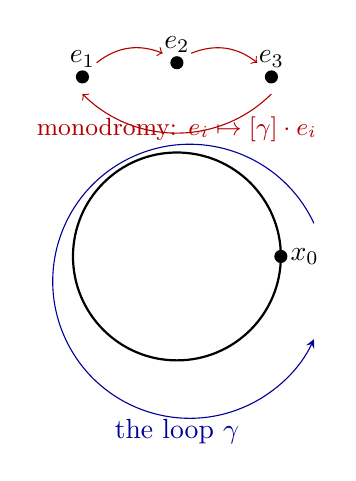
\begin{tikzpicture}[scale=1.2]
			\draw[thick] (0,0) circle (1.1);
			\filldraw (1.1,0) circle (1.8pt) node[right] {$x_0$};
			\draw[->,>=stealth,blue!60!black] (1.45,0.35) arc (25:335:1.45);
			\node[blue!60!black] at (0,-1.85) {the loop $\gamma$};
			\filldraw (-1,1.9) circle (1.8pt) node[above] {$e_1$};
			\filldraw (0,2.05) circle (1.8pt) node[above] {$e_2$};
			\filldraw (1,1.9) circle (1.8pt) node[above] {$e_3$};
			\draw[->,red!70!black] (-0.85,2.05) to[bend left=30] (-0.15,2.15);
			\draw[->,red!70!black] (0.15,2.15) to[bend left=30] (0.85,2.05);
			\draw[->,red!70!black] (1.0,1.72) to[bend left=45] (-1.0,1.72);
			\node[red!70!black] at (0,1.35) {\small monodromy: $e_i\mapsto[\gamma]\cdot e_i$};
		\end{tikzpicture}
		\caption{Monodromy: lifting the loop $\gamma$ from each point of the fiber permutes the fiber.
			This permutation representation is the topological shadow of the Galois action on roots.}
	\end{figure}
	
	\begin{definition}[Deck transformations]
		A \textbf{deck transformation} of $p:E\to X$ is a homeomorphism $\varphi:E\to E$ with
		$p\circ\varphi=p$; they form the \textbf{deck group} $\Deck(p)=\Aut(E/X)$.
	\end{definition}
	
	\begin{proposition}\label{prop:deck-free}
		$\Deck(p)$ acts freely on each fiber; if $E$ is connected, a deck transformation is determined by
		its value at a single point; hence $|\Deck(p)|\le|p^{-1}(x)|$ for every $x$.
	\end{proposition}
	\begin{proof}
		A deck transformation $\varphi$ is a lift of $p:E\to X$ itself (since $p\circ\varphi=p$); two deck
		maps agreeing at one point are equal by the uniqueness argument of
		Proposition~\ref{prop:path-lifting} applied to the identity path and connectedness of $E$. Freeness:
		if $\varphi(e)=e$ then $\varphi=\id$ by the same uniqueness, so no nontrivial deck map fixes a fiber
		point.
	\end{proof}
	
	\begin{example}
		$\Deck(\R\to S^1)=\{t\mapsto t+m:m\in\Z\}\cong\Z$; $\Deck(p_n:S^1\to S^1)=\{z\mapsto z\zeta:\zeta\in\mu_n\}\cong\Z/n$;
		$\Deck(\R^2\to T^2)\cong\Z^2$. In each case $|\Deck|$ equals the fiber size: these coverings are
		\emph{maximally symmetric}.
	\end{example}
	
	\begin{definition}[Universal covering]
		A covering $p:\tilde X\to X$ with $\tilde X$ simply connected ($\pi_1=0$) is a \textbf{universal
			covering}. Examples: $\R\to S^1$, $\R^2\to T^2$, $\R^n\to T^n$; existence holds for spaces that are
		path-connected, locally path-connected, and semi-locally simply connected.
	\end{definition}
	
	\begin{proposition}[Deck group of the universal cover]\label{prop:deck-universal}
		If $p:\tilde X\to X$ is a universal covering, then $\Deck(p)\cong\pi_1(X,x_0)$; more precisely the
		monodromy action identifies the fiber $p^{-1}(x_0)$ with $\pi_1(X,x_0)$ and the deck action with
		left multiplication.
	\end{proposition}
	\begin{proof}[Proof idea]
		Since $\tilde X$ is simply connected, lifts of loops are unique and the endpoint map
		$[\gamma]\mapsto\tilde\gamma_{e_0}(1)$ is a bijection $\pi_1(X,x_0)\to p^{-1}(x_0)$ (surjectivity:
		join $e_0$ to any $e$ by a path in $\tilde X$ and project). Each $g\in\pi_1$ then determines a unique
		deck map sending $e_0$ to $[\gamma]\cdot e_0$ (Proposition~\ref{prop:deck-free} plus lifting of the
		whole covering from the universal property), and composition matches group multiplication.
	\end{proof}
	
	\begin{theorem}[$\pi_1(S^1)\cong\Z$]\label{thm:pi1-S1}
		The map $\deg:[\gamma]\mapsto\tilde\gamma(1)$, where $\tilde\gamma$ is the lift of $\gamma$ (based at
		$1\in S^1$) starting at $0\in\R$ along $p:\R\to S^1$, is a well-defined group isomorphism
		$\pi_1(S^1,1)\xrightarrow{\ \cong\ }\Z$.
	\end{theorem}
	\begin{proof}
		\emph{Well-defined:} $\tilde\gamma(1)\in p^{-1}(1)=\Z$; homotopic loops have lifts with equal
		endpoints (Proposition~\ref{prop:homotopy-lifting}). \emph{Homomorphism:} the lift of $\gamma*\eta$
		is the lift of $\gamma$ followed by the translate by $\deg(\gamma)$ of the lift of $\eta$ (both are
		lifts of the second half with the same start), so $\deg(\gamma*\eta)=\deg(\gamma)+\deg(\eta)$.
		\emph{Surjective:} $\gamma_n(t)=e^{2\pi i n t}$ lifts to $t\mapsto nt$, ending at $n$.
		\emph{Injective:} if $\deg([\gamma])=0$ then $\tilde\gamma$ is a loop in $\R$ based at $0$; $\R$
		contractible gives a null-homotopy $\tilde H$; projecting, $p\circ\tilde H$ is a null-homotopy of
		$\gamma$ rel basepoint. Hence $\deg$ is an isomorphism.
	\end{proof}
	
	% ══════════════════════════════════════════════
	\section{Classification of Coverings and the Galois Dictionary}
	% ══════════════════════════════════════════════
	
	\begin{theorem}[Classification of coverings]\label{thm:classification}
		Let $X$ be path-connected, locally path-connected, and semi-locally simply connected, with basepoint
		$x_0$. The functor
		\[
		(E\xrightarrow{p} X)\ \longmapsto\ \big(p^{-1}(x_0),\ \text{monodromy}\big)
		\]
		is an equivalence between the category of coverings of $X$ and the category of $\pi_1(X,x_0)$-sets.
		Under it: connected coverings $\leftrightarrow$ transitive $\pi_1$-sets; based connected coverings
		(up to based isomorphism) $\leftrightarrow$ subgroups of $\pi_1(X,x_0)$, via
		$H=p_*\pi_1(E,e_0)=\{[\gamma]:[\gamma]\cdot e_0=e_0\}$ (the stabilizer of $e_0$).
	\end{theorem}
	\begin{proof}[Construction and proof idea]
		Inverse functor: given a $\pi_1$-set $S$, form $E_S=(\tilde X\times S)/\pi_1$ with the diagonal action
		$[\gamma]\cdot(\tilde x,s)=(\tilde x\cdot[\gamma]^{-1},[\gamma]\cdot s)$ using the universal cover
		$\tilde X$; the projection $E_S\to X$ is a covering with fiber $S$ and the prescribed monodromy.
		Checking the two functors are mutually inverse uses Proposition~\ref{prop:deck-universal} and the
		unique-lifting properties. The stabilizer description follows from the definition of monodromy:
		loops fixing $e_0$ are exactly those lifting to loops at $e_0$, i.e.\ $p_*\pi_1(E,e_0)$.
	\end{proof}
	
	\begin{definition}[Normal (Galois) covering]
		A connected covering $p:E\to X$ is \textbf{normal} (or \textbf{Galois}) if
		$p_*\pi_1(E,e_0)\trianglelefteq\pi_1(X,x_0)$; equivalently $\Deck(p)$ acts transitively on each fiber.
	\end{definition}
	
	\begin{proposition}[Topological Galois correspondence]\label{prop:galois-corr}
		For $X$ as above, with $\pi=\pi_1(X,x_0)$: connected coverings of $X$ (up to equivalence)
		correspond to conjugacy classes of subgroups $H\le\pi$; normal coverings to normal subgroups; and
		for the covering $E_H$ corresponding to $H$,
		\[
		\Deck(E_H)\ \cong\ N_\pi(H)/H,
		\]
		so in particular the universal cover (corresponding to $H=\{1\}$) has $\Deck\cong\pi$, and a Galois
		covering has $\Deck\cong\pi/H$.
	\end{proposition}
	\begin{proof}[Proof idea]
		From Theorem~\ref{thm:classification}, $\Deck(E_H)$ equals the $\pi_1$-set automorphisms of the
		transitive set $\pi/H$, which are right multiplications by elements normalizing $H$, modulo those
		acting trivially ($H$ itself): $N_\pi(H)/H$. Transitivity of the deck action $\iff$ normality of $H$
		is the same computation.
	\end{proof}
	
	\begin{example}[Coverings of $S^1$ classified]
		Subgroups of $\Z$ are $n\Z$; the connected covering for $n\Z$ is $p_n:S^1\to S^1$, $z\mapsto z^n$
		(for $n\ge1$), with $\Deck\cong\Z/n$; all are normal since $\Z$ is abelian; the universal cover is
		$n=0$: $\R\to S^1$ with $\Deck\cong\Z$. Compare: finite extensions of a field classified by
		subgroups of its Galois group in the finite case --- the same shape.
	\end{example}
	
	\begin{remark}[The dictionary: topology $\leftrightarrow$ Galois theory]\label{rem:dictionary}
		\begin{center}\small
			\begin{tabular}{|l|l|}
				\hline
				\textbf{Topology (this session)} & \textbf{Galois theory (Acts II, VI; S35)} \\
				\hline
				Covering $p:E\to X$ & Field extension $L/K$ \\
				Connected / finite-sheeted covering & Field extension / finite extension \\
				Universal cover $\tilde X$ & Separable closure $K^{\mathrm{sep}}$ \\
				Deck group $\Deck(p)$ & Galois group $\Gal(L/K)$ \\
				Normal (Galois) covering & Galois extension \\
				$\pi_1(X,x_0)$ & Absolute Galois group $G_K$ (S16) \\
				Monodromy action on the fiber & Galois action on roots / on the fiber \\
				Index $[\pi_1:H]$ & Degree $[L:K]$ \\
				\hline
			\end{tabular}
		\end{center}
		Grothendieck's move (S35): for a scheme there is no classical topology, but the \emph{category of
			finite \'etale covers} still exists; define $\pi_1^{\text{\'et}}$ by demanding the same
		classification theorem (finite covers $\leftrightarrow$ finite continuous $\pi_1$-sets). For
		$X=\Spec K$ this recovers exactly $G_K$; for nice complex varieties $\pi_1^{\text{\'et}}$ is the
		profinite completion of the topological $\pi_1$ (Riemann existence theorem).
	\end{remark}
	
	\begin{remark}[Profinite nature; scope of this session]\label{rem:profinite-scope}
		Because only \emph{finite} covers are remembered algebraically, $\pi_1^{\text{\'et}}$ is a
		\textbf{profinite group} (S34): an inverse limit of finite deck groups, e.g.\
		$\pi_1^{\text{\'et}}(\Spec\Q)=G_\Q=\varprojlim \Gal(L/\Q)$. Monodromy of an infinite Galois extension
		is the inverse limit of finite permutation representations. Scope note: we deliberately stop here ---
		no homology, no higher homotopy groups --- because the course needs exactly this categorical
		pattern: \emph{covers $\leftrightarrow$ $\pi_1$-sets}.
	\end{remark}
	
	\begin{remark}[Monodromy as evaluation]
		Lifting a loop and watching the fiber permute is \emph{analytic continuation of a point along a
			loop}: the fiber point is a ``solution'' (a root, a sheet) and the loop evaluates how solutions
		transform. This is the topological ancestor of ``point $=$ morphism'' (S29, S54): a point of the
		fiber over $x$ is a map into $X$ together with a chosen lift, and monodromy is the action of loops
		on such choices.
	\end{remark}
	
	% ══════════════════════════════════════════════
	\section{Exercises}
	% ══════════════════════════════════════════════
	\begin{exercise}
		Write out the explicit homotopies proving Proposition~\ref{prop:pi1-group} (identity, associativity,
		inverse) without hand-waving reparametrizations.
	\end{exercise}
	\begin{exercise}
		Prove Proposition~\ref{prop:basepoint} in full: well-definedness, homomorphism property, and
		$\beta_{\alpha^{-1}}=(\beta_\alpha)^{-1}$. Show $\beta_\alpha$ depends only on the path-homotopy
		class of $\alpha$.
	\end{exercise}
	\begin{exercise}
		Prove $\pi_1(X\times Y)\cong\pi_1(X)\times\pi_1(Y)$ carefully and deduce $\pi_1(T^n)\cong\Z^n$.
	\end{exercise}
	\begin{exercise}
		Show that a disk $D^2$, a cone, and $\R^n$ are contractible; conclude they are simply connected.
		Using Theorem~\ref{thm:pi1-S1}, prove $S^1$ is \emph{not} contractible.
	\end{exercise}
	\begin{exercise}
		For $p_n:S^1\to S^1$, $z\mapsto z^n$: describe the fiber over $1$, the monodromy permutation of a
		generator, and $\Deck(p_n)$; verify $|\Deck|=n=$ number of sheets.
	\end{exercise}
	\begin{exercise}
		Prove Proposition~\ref{prop:path-lifting} in full detail, including the Lebesgue-number subdivision
		for existence and the open-closed argument for uniqueness.
	\end{exercise}
	\begin{exercise}
		For $p:\R\to S^1$: prove $\Deck(p)\cong\Z$ explicitly and identify the monodromy homomorphism
		$\pi_1(S^1)\to\Deck(p)$ under the isomorphism of Theorem~\ref{thm:pi1-S1}.
	\end{exercise}
	\begin{exercise}
		Reconstruct Theorem~\ref{thm:pi1-S1} from scratch using only the three lifting properties (path,
		homotopy, uniqueness): define $\deg$, prove it is a well-defined bijective homomorphism.
	\end{exercise}
	\begin{exercise}
		Classify connected coverings of $S^1$ up to equivalence of coverings; match each with a subgroup of
		$\Z$; decide which are normal and compute their deck groups via
		Proposition~\ref{prop:galois-corr}.
	\end{exercise}
	\begin{exercise}
		Show that a map homotopic to a constant induces the trivial homomorphism on $\pi_1$; deduce that
		$\pi_1$ cannot distinguish a point from $\R^n$ (motivating homology and higher invariants, not
		covered here).
	\end{exercise}
	\begin{exercise}[The dictionary at work]
		Translate into covering language: (i) the quadratic extension $\Q(\sqrt d)/\Q$; (ii) the cyclotomic
		extension $\Q(\zeta_n)/\Q$; (iii) the universal cover of $S^1$. Then translate back: the covering
		$p_2:S^1\to S^1$; the trivial covering $X\times\{1,2\}\to X$.
	\end{exercise}
	\begin{exercise}[Challenge]
		State (without proof) that $\pi_1(S^1\vee S^1)$ is free on two generators; describe its universal
		covering as a graph (the Cayley graph of $F_2$) and explain why it is simply connected.
	\end{exercise}
	
	% ══════════════════════════════════════════════
	\section*{Where This Session Feeds the Course}
	\addcontentsline{toc}{section}{Where This Session Feeds the Course}
	% ══════════════════════════════════════════════
	\begin{itemize}
		\item \textbf{Depends on:} P2 (topology, connectedness, compactness of $[0,1]$); P1 (group language,
		free groups preview).
		\item \textbf{Feeds:} S34 (profinite groups as inverse limits of deck groups); S35 (\'etale $\pi_1$
		and Grothendieck's correspondence: the same classification theorem with \'etale covers);
		S16 ($G_\Q$ as profinite $\pi_1$ of $\Spec\Q$); S60 (Dessins d'Enfants: monodromy of covers of
		$\PP^1\setminus\{0,1,\infty\}$); Act~VII (topoi internalize ``covers $\leftrightarrow$ $\pi_1$-sets'').
		\item \textbf{Unifying thread:} a covering is a space of points over points; monodromy is evaluation
		along loops; the Galois correspondence is the classification of point-systems over a base.
	\end{itemize}
	
	\subsection*{References for this session}
	\begin{enumerate}[label={[\arabic*]}]
		\item Hatcher, A. \emph{Algebraic Topology}, ch.0--1 (selected: $\pi_1$, coverings, lifting).
		\item May, J.P. \emph{A Concise Course in Algebraic Topology}, ch.1--3 (selected).
		\item Munkres, J.R. \emph{Topology}, \S51--54 (fundamental group and coverings).
		\item Szamuely, T. \emph{Galois Groups and Fundamental Groups}, ch.2 (the Galois-correspondence
		viewpoint and the bridge to \'etale $\pi_1$).
	\end{enumerate}
	
	\vspace{1.5em}
	\begin{center}
		\rule{0.6\textwidth}{0.4pt}\\[0.5em]
		\textit{End of Session P3 --- the Prelude is complete; next: Act 0, Session S1, Rings, Ideals, and Spectra}
	\end{center}
	
\end{document}